\begin{figure}[!ht]
    \centering
    \subfloat[Bayes]{
        \label{abortBayes}
        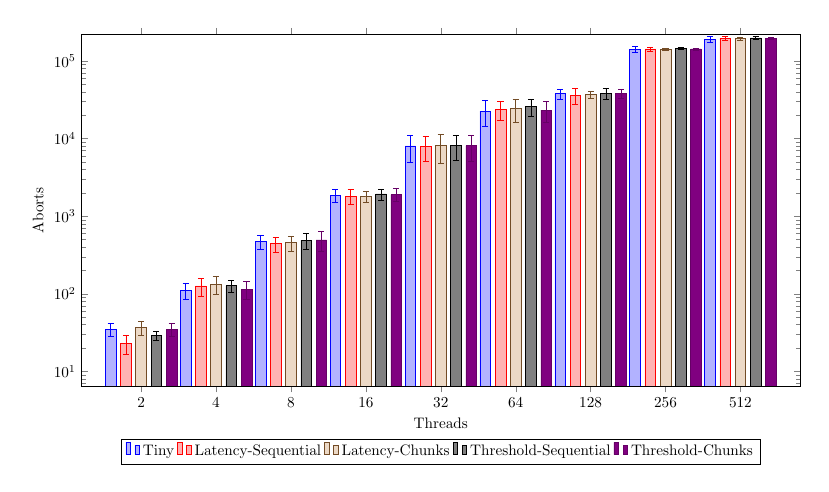
\begin{tikzpicture}[scale=0.55, baseline]
        \begin{axis}[
            ymode=log,
            width=1.5 \linewidth,
            height=0.8 \linewidth,
            %media de tempo intruder
            ybar=3pt,
            %enlargelimits=0.10,
            legend style={at={(0.5,-0.15)}, anchor=north, legend columns=-1},
            ylabel=Aborts,
            xlabel=Threads,
            symbolic x coords={1, 2, 4, 8, 16, 32, 64, 128, 256, 512},
            xtick=data,
            ymin=0,
            ymax=220000,
            bar width=7pt,
            % nodes near coords,
            nodes near coords align={vertical},
        ]
        \addplot+[error bars,y dir=both, y explicit] coordinates {
            (1,0.0)+-(1,0.0) (2,35.0)+-(2,6.72) (4,111.0)+-(4,25.13) (8,470.6)+-(8,101.19) (16,1858.6)+-(16,343.71) (32,8018.2)+-(32,3060.82) (64,22527.4)+-(64,8121.85) (128,37743.2)+-(128,5565.49) (256,141872.2)+-(256,13892.27) (512,191436.8)+-(512,17258.39)
        };
        \addplot+[error bars,y dir=both, y explicit] coordinates {
            (1,0.0)+-(1,0.0) (2,23.0)+-(2,6.23) (4,126.0)+-(4,32.76) (8,440.6)+-(8,99.82) (16,1800.2)+-(16,399.13) (32,7936.18)+-(32,2798.23) (64,23847.2)+-(64,6522.42) (128,35938.5)+-(128,8262.18) (256,142628.8)+-(256,7947.57) (512,196582.3)+-(512,9788.9)
        };
        \addplot+[error bars,y dir=both, y explicit] coordinates {
            (1,0.0)+-(1,0.0) (2,37.0)+-(2,7.7) (4,131.4)+-(4,34.43) (8,455.22)+-(8,97.63) (16,1798.25)+-(16,285.341) (32,8134.4)+-(32,3281.67) (64,24227.4)+-(64,7812.5) (128,36972.9)+-(128,3907.18) (256,141539.2)+-(256,3362.2) (512,192748.4)+-(512,10239.43)
        };
        \addplot+[error bars,y dir=both, y explicit] coordinates {
            (1,0.0)+-(1,0.0) (2,29.0)+-(2,3.55) (4,127.0)+-(4,22.63) (8,487.9)+-(8,111.47) (16,1929.2)+-(16,317.1) (32,8063.21)+-(32,2840.32) (64,25728.67)+-(64,6565.8) (128,38082.222)+-(128,5736.93) (256,144284.24)+-(256,3475.15) (512,197398.8)+-(512,7834.42)
        };
        \addplot+[error bars,y dir=both, y explicit] coordinates {
            (1,0.0)+-(1,0.0) (2,35.0)+-(2,6.72) (4,114.94)+-(4,29.3) (8,494.33)+-(8,137.9) (16,1898.36)+-(16,364.82) (32,8082.64)+-(32,3019.92) (64,23189.6)+-(64,6989.99) (128,37964.7)+-(128,5387.7) (256,142367.33)+-(256,3478.75) (512,195893.8)+-(512,6746.09)
        };
        \legend {Tiny, Latency-Sequential, Latency-Chunks, Threshold-Sequential, Threshold-Chunks}
        \end{axis}
        \end{tikzpicture}
    }
    
    \subfloat[Intruder]{
        \label{abortIntruder}
        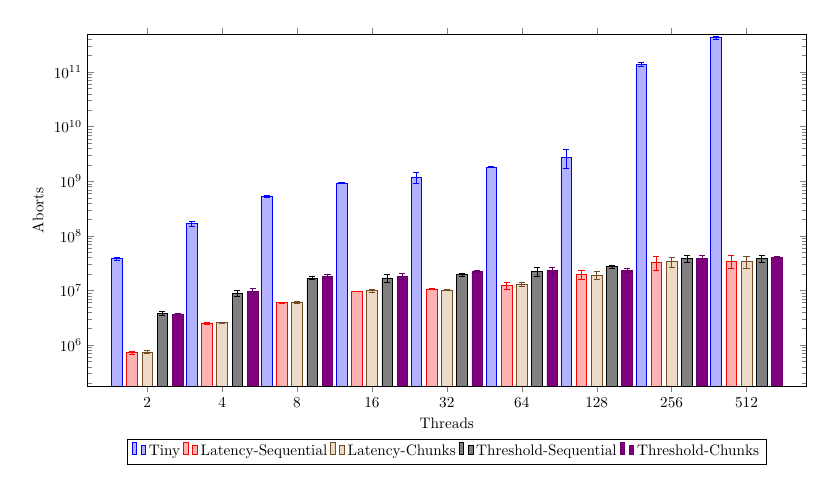
\begin{tikzpicture}[scale=0.55, baseline]
        \begin{axis}[
            ymode=log,
            width=1.5 \linewidth,
            height=0.8 \linewidth,
            %media de tempo intruder
            ybar=3pt,
            %enlargelimits=0.10,
            legend style={at={(0.5,-0.15)}, anchor=north, legend columns=-1},
            ylabel=Aborts,
            xlabel=Threads,
            symbolic x coords={1, 2, 4, 8, 16, 32, 64, 128, 256, 512},
            xtick=data,
            ymin=0,
            ymax=490000000000,
            bar width=7pt,
            % nodes near coords,
            nodes near coords align={vertical},
        ]
        \addplot+[error bars,y dir=both, y explicit] coordinates {
            (1,0.0)+-(1,0.0) (2,38000260.8)+-(2,2949711.678076852) (4,166325696.4)+-(4,18557044.648063533) (8,529197870.6)+-(8,22132676.255908735) (16,924927047.6)+-(16,24358107.18760883) (32,1183579117.4)+-(32,270222169.9344623) (64,1831169740.8)+-(64,62890886.257802844) (128,2763435636.6)+-(128,1003746150.3805901) (256,138779112147.6)+-(256,10430244205.851603) (512,431443096033.6)+-(512,28705521954.994297) 
        };
        \addplot+[error bars,y dir=both, y explicit] coordinates {
            (1,0.0)+-(1,0.0) (2,724967.4)+-(2,38086.07014959669) (4,2505616.2)+-(4,79429.60770745378) (8,6012716.4)+-(8,169677.49348290125) (16,9639253.0)+-(16,142573.7883104745) (32,10568731.0)+-(32,292443.9680909832) (64,12171771.4)+-(64,1784435.4526392485) (128,19342142.8)+-(128,3669581.5184994815) (256,32980054.25)+-(256,9356623.644361822) (512,34119006.5)+-(512,8983159.5)
        };
        \addplot+[error bars,y dir=both, y explicit] coordinates {
             (1,0.0)+-(1,0.0) (2,745630.2)+-(2,40338.85590792084) (4,2559770.6)+-(4,81679.883166175) (8,6127472.777777778)+-(8,267489.386445634) (16,9889825.3)+-(16,755124.9867329315) (32,10236117.3)+-(32,288410.38292407227) (64,13078693.1)+-(64,982436.3361754746) (128,19063545.666666668)+-(128,2925827.5185046173) (256,33704832.6)+-(256,6772680.448815952) (512,34183921.0)+-(512,8274893.22) 
        };
        \addplot+[error bars,y dir=both, y explicit] coordinates {
            (1,0.0)+-(1,0.0) (2,3808172.2)+-(2,327085.8815720422) (4,9023407.8)+-(4,1123234.4180183227) (8,16872564.2)+-(8,1114383.5354166715) (16,17004377.2)+-(16,2666034.739783216) (32,19648666.0)+-(32,1287522.1930899676) (64,22307089.8)+-(64,4029768.617032169) (128,27162139.0)+-(128,1504557.0) (256,38132893.15)+-(256,4958389.304) (512,37984673.0)+-(512,5282793.33)
        };
        \addplot+[error bars,y dir=both, y explicit] coordinates {
            (1,0.0)+-(1,0.0) (2,3578932.78)+-(2,176854.86) (4,9738434.34)+-(4,1124342.85) (8,17928374.6)+-(8,1573847.9) (16,18301736.6)+-(16,2468736.987185277) (32,22436982.0)+-(32,1106602.0) (64,23420167.2)+-(64,3281430.727250502) (128,23366253.0)+-(128,1919489.0) (256,38736187.88)+-(256,5748878.34) (512,39763372.723)+-(512,3174827.12)
        };
        \legend {Tiny, Latency-Sequential, Latency-Chunks, Threshold-Sequential, Threshold-Chunks}
        \end{axis}
        \end{tikzpicture}
    }

    \subfloat[Kmeans]{
        \label{abortKmeans}
        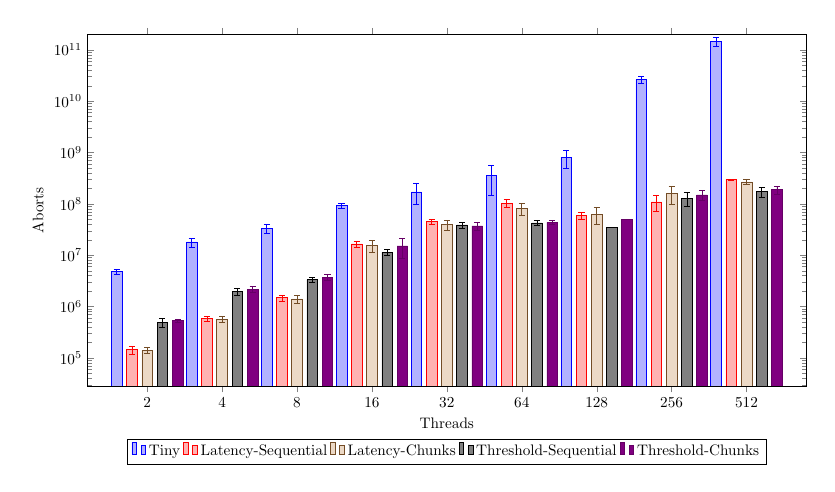
\begin{tikzpicture}[scale=0.55, baseline]
        \begin{axis}[
            ymode=log,
            width=1.5 \linewidth,
            height=0.8 \linewidth,
            %media de tempo intruder
            ybar=3pt,
            %enlargelimits=0.10,
            legend style={at={(0.5,-0.15)}, anchor=north, legend columns=-1},
            ylabel=Aborts,
            xlabel=Threads,
            symbolic x coords={1, 2, 4, 8, 16, 32, 64, 128, 256, 512},
            xtick=data,
            ymin=0,
            ymax=200000000000,
            bar width=7pt,
            % nodes near coords,
            nodes near coords align={vertical},
        ]
        \addplot+[error bars,y dir=both, y explicit] coordinates {
            (1,0.0)+-(1,0.0) (2,4797421.2)+-(2,479774.7418784778) (4,18101846.8)+-(4,3591708.3539415835) (8,33182746.2)+-(8,6732288.556793311) (16,93057923.8)+-(16,9863144.322012922) (32,171442797.6)+-(32,74829388.10384364) (64,359745893.2)+-(64,213043475.04545623) (128,807753260.2)+-(128,310719932.9857997) (256,26569175006.4)+-(256,4470117158.120106) (512,146296330743.6)+-(512,26886172215.929005) 
        };
        \addplot+[error bars,y dir=both, y explicit] coordinates {
            (1,0.0)+-(1,0.0) (2,144295.6)+-(2,24864.282793597726) (4,579330.6)+-(4,68221.2484981036) (8,1486520.2)+-(8,200173.524986098) (16,16580311.4)+-(16,2227873.6890443857) (32,45063610.6)+-(32,5053643.0020858655) (64,103498202.6)+-(64,18052939.09375) (128,59441333.6)+-(128,8917614.717479235) (256,109146323.8)+-(256,36880499.382352196) (512,294773353.4)+-(512,3281309.7536428105)
        };
        \addplot+[error bars,y dir=both, y explicit] coordinates {
             (1,0.0)+-(1,0.0) (2,141609.1)+-(2,19957.913370139675) (4,570320.1)+-(4,69142.6626511447) (8,1412101.5)+-(8,239771.55806068826) (16,15454899.8)+-(16,3814349.1856658272) (32,39591108.222222224)+-(32,9286948.71968007) (64,81659510.1)+-(64,21584431.489666473) (128,62701912.9)+-(128,22625798.149042867) (256,157892521.1)+-(256,60541141.358650364) (512,267641468.75)+-(512,32356420.707834) 
        };
        \addplot+[error bars,y dir=both, y explicit] coordinates {
            (1,0.0)+-(1,0.0) (2,489474.6)+-(2,95557.56667391652) (4,1982817.6)+-(4,324496.7328282983) (8,3338695.4)+-(8,339537.1836017964) (16,11407592.4)+-(16,1467579.9615602007) (32,38923440.666666664)+-(32,5311247.22872386) (64,42424191.0)+-(64,4907763.0) (128,34826711.0)+-(128,578473.0) (256,128783746.63)+-(256,37482783.86) (512,173847878.28)+-(512,37384778.0)
        };
        \addplot+[error bars,y dir=both, y explicit] coordinates {
            (1,0.0)+-(1,0.0) (2,528574.7)+-(2,29384.0) (4,2157923.0)+-(4,283746.0) (8,3736425.62)+-(8,429388.0) (16,15208687.0)+-(16,6397145.233711557) (32,37279545.0)+-(32,6425946.0) (64,43456253.0)+-(64,3849829.0) (128,49875516.0)+-(128,675193.0) (256,148983127.32)+-(256,31827833.0) (512,187678278.0)+-(512,32738943.73)
        };
        \legend {Tiny, Latency-Sequential, Latency-Chunks, Threshold-Sequential, Threshold-Chunks}
        \end{axis}
        \end{tikzpicture}
    }
    
    \caption{Aborts em NUMA variando o número de \emph{threads}.}
    \label{abort}

\end{figure}
